%%%%%%%%%%%%%%%%%%%%%%%%%%%%
\section{Introduction}
\label{sec:Introduction}
%%%%%%%%%%%%%%%%%%%%%%%%%%%%

For many years, the existence of pink elephants has been hypothesised. Flamingoes are pink, penguins are not pink, so there must be pink elephants as well.

\autoref{NotAPinkElephant} shows what a pink elephant does not look like:
\begin{figure}[h]
\begin{center}
	\subfigure[A grey elephant. Definitely not pink.]{\label{GreyElephant} 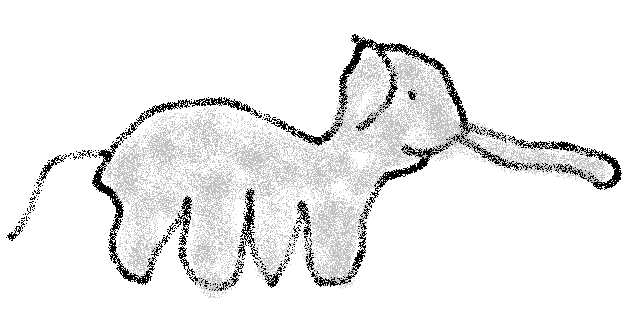
\includegraphics[width=0.33\textwidth]{GreyElephant} }
	\subfigure[A common misconception is that pinkuins are pink. This is not true, as they are not elephants.]{\label{Pinkuin} 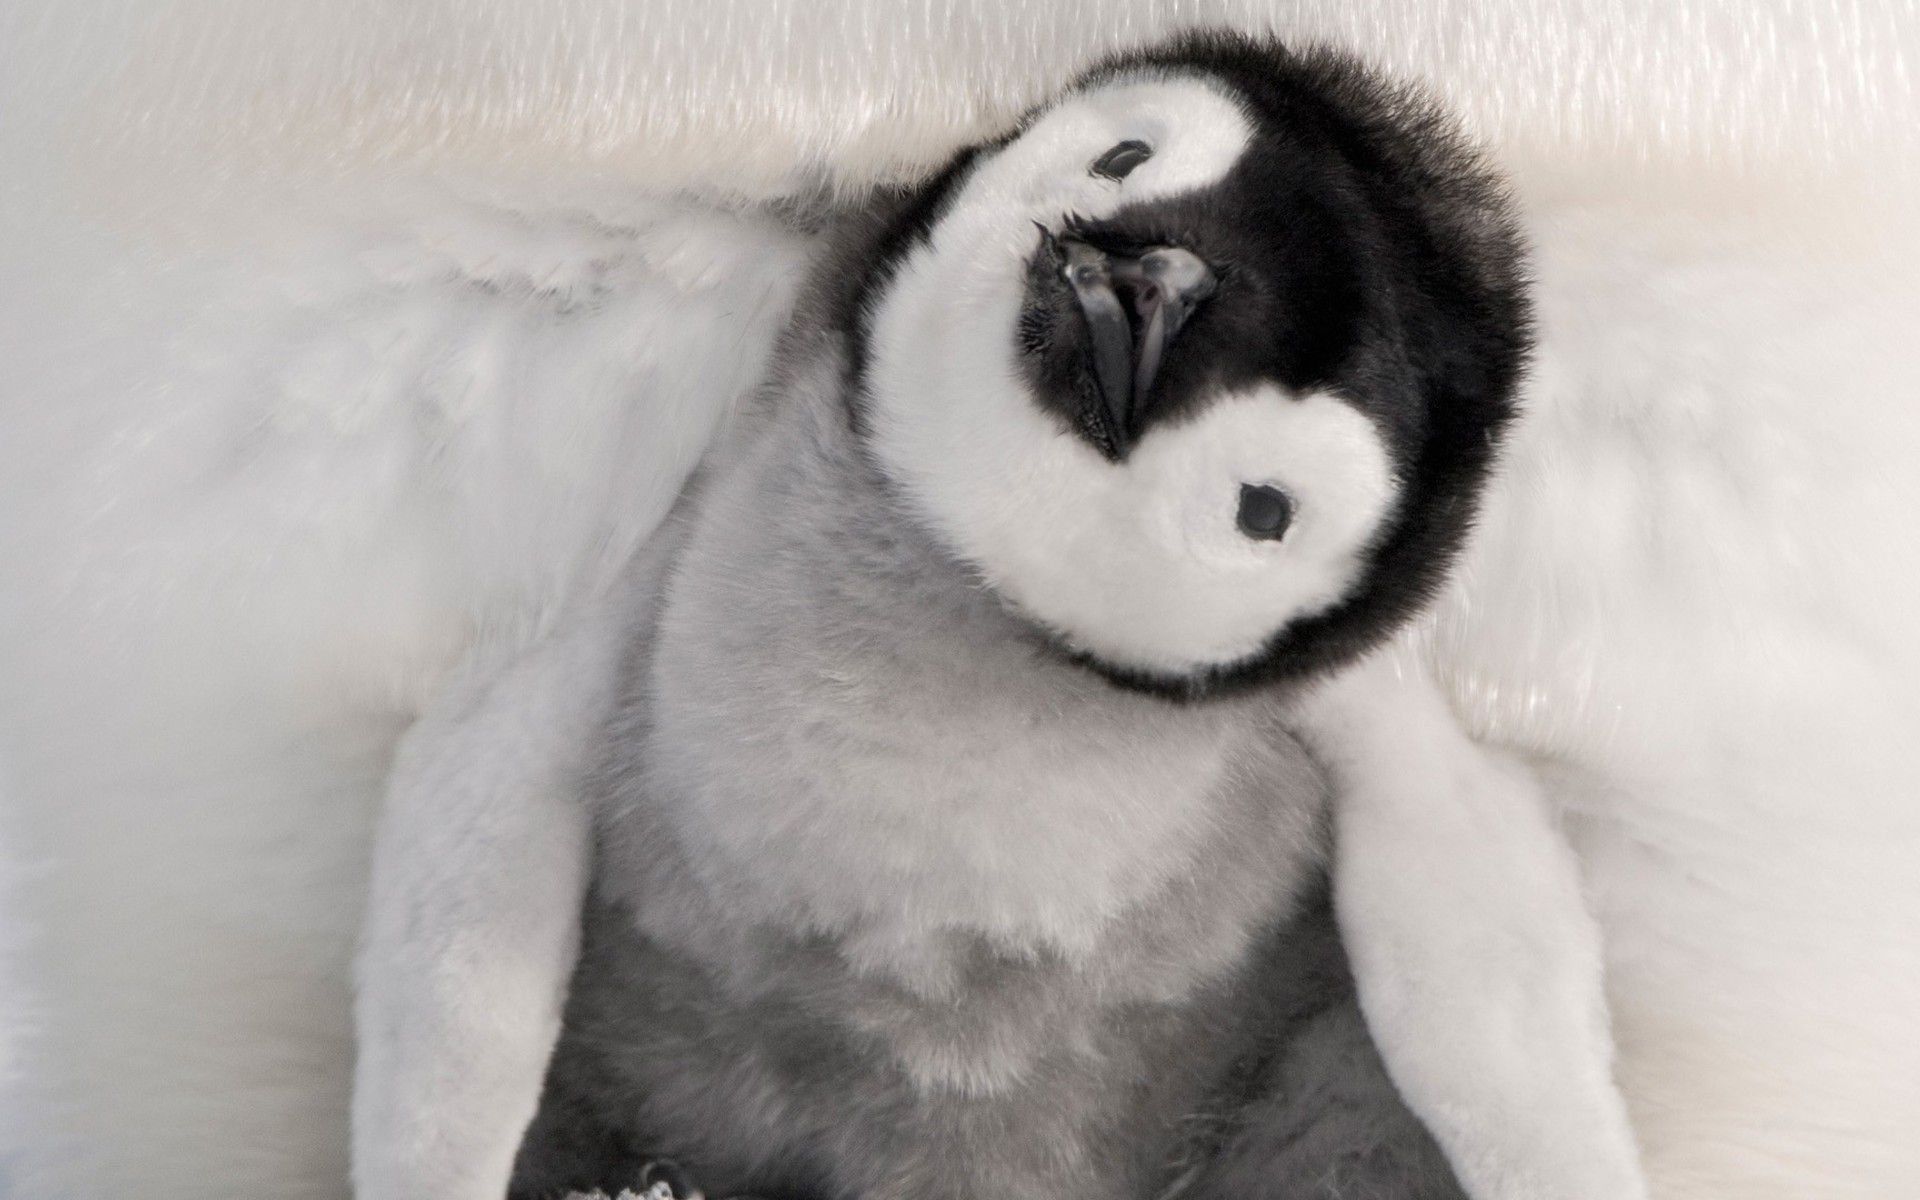
\includegraphics[width=0.33\textwidth]{Pinkuin} }
	\caption{Non-pink non-elephants.}
	\label{NotAPinkElephant}
\end{center}
\end{figure} 
